The \las~Detector Control System (DCS) may be divided in two parts. The first component is internal.  It is used to drive the system and to collect information. The second part is related to ATLAS. The data collected are transmitted to the control room (online survey) and stored in a database.

\subsubsection{Internal DCS}

The internal part of the \las~DCS is driven by the Laser Independent COntrol Remote NEtwork (LICORNE) (Fig. \ref{fig:laslicorne}). The communication between the modules concerned (LicMot, LicPhd, LicPmt, LASCAR,LASER pump) is performed through ethernet (except for the LASER pump, where an RS232 connexion is used). The heart of the system is a 32-bits PIC microcontroller PIC32MX795F512L (C programming langage) from Microchip \cite{ref:picmicro}. All modules use DHCP client for IP Address resolution. Web interfaces (based on Java) have been developed to set orders or read information in an easy way. Some illustration are given in appendix A, where web pages related to LicPhd, LicMot, LicPmt and LASCAR are displayed. It is possible to set parameters such as the PMT high voltages or the filter wheel position, to perform actions such as moving the filter wheel, and to read parameters such as temperatures in the cassettes or humidity level in the PHOCAL box.


\begin{figure}[htbp]
\centering
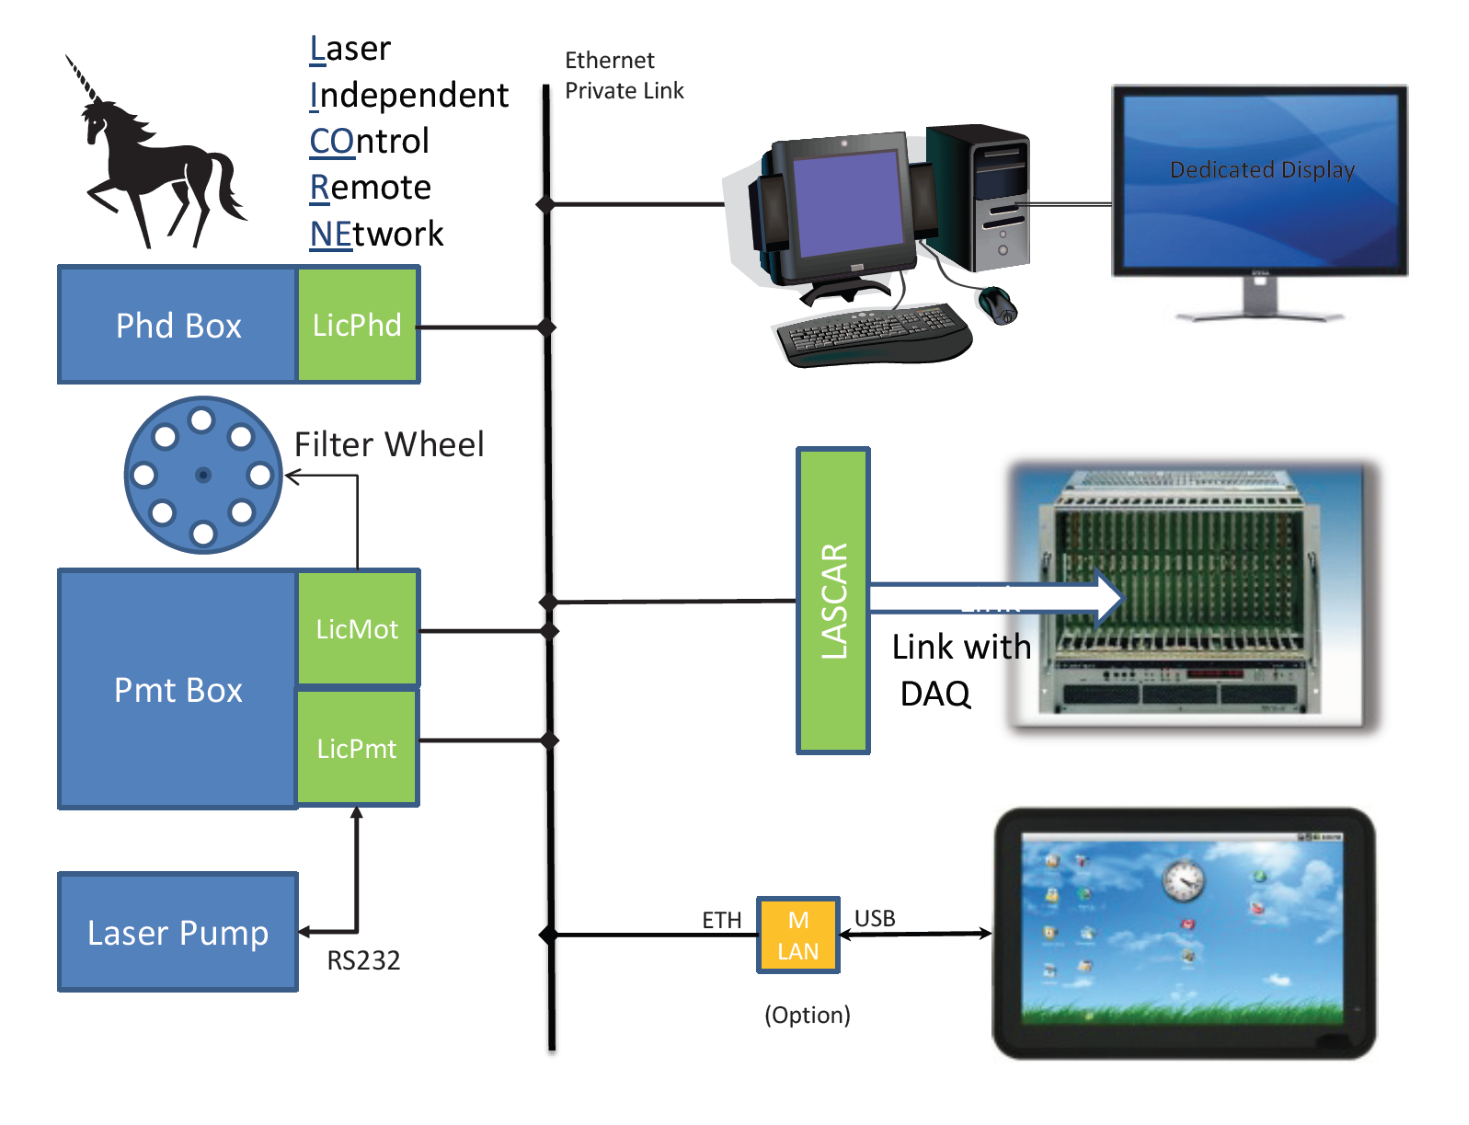
\includegraphics[width=9cm]{figures/licorne.pdf}
\caption{Scheme of the LICORNE system used to drive the internal DCS side of the \las}\label{fig:laslicorne}
\end{figure}

\subsubsection{ATLAS DCS}

A scheme of the ATLAS-DCS part of the \las~system is given on Fig. \ref{fig:lasdcs}. Data collected by LICORNE are dumped on a PC located in USA15 and retrieved by a DIM server. Information are then transmitted to a PVSS DIM server used to publish and store the data in a database.

\begin{figure}[htbp]
\centering
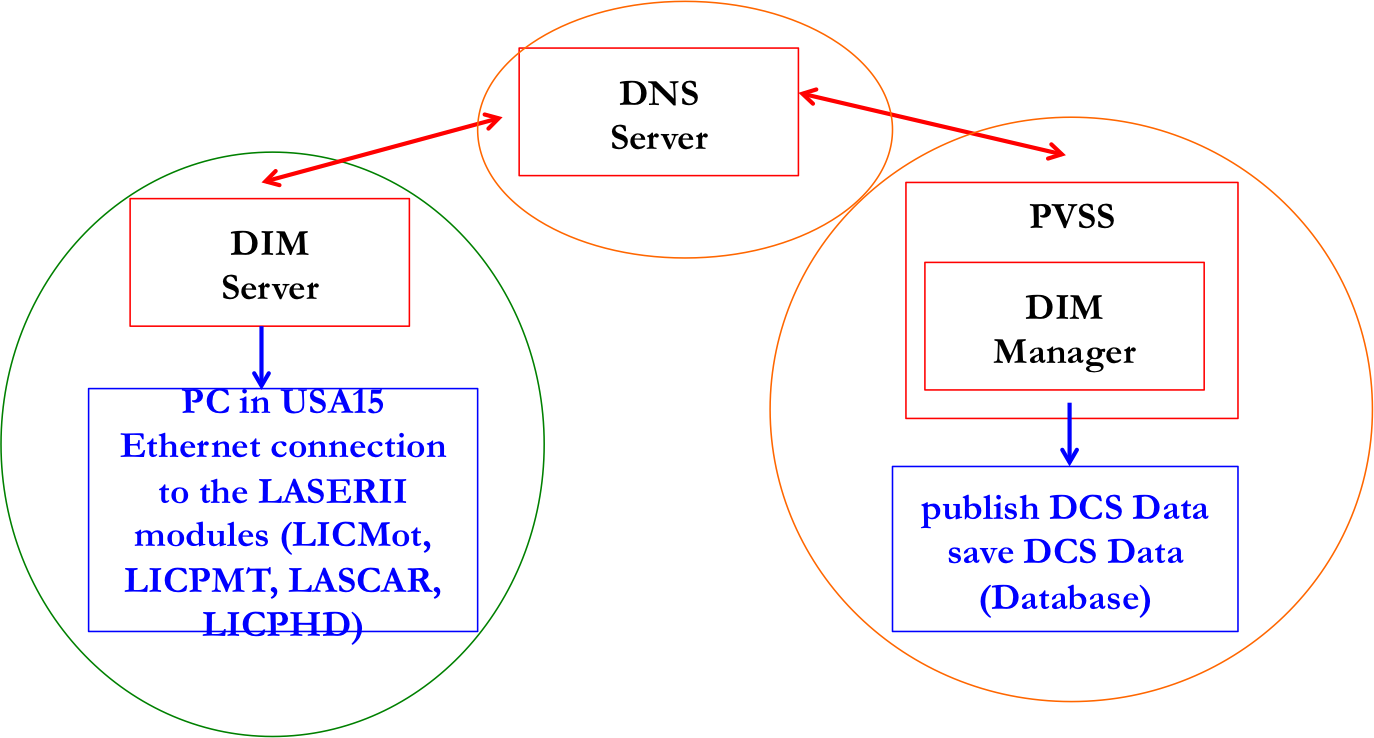
\includegraphics[width=9cm]{figures/dcs_scheme.png}
\caption{Scheme of the DCS ATLAS-side of the \las}\label{fig:lasdcs}
\end{figure}

There are two ways to access DCS data. In real-time information are available in ATLAS control room through PVSS panels (see appendix B) and should be used by the shifter to estimate the status of the \laser~and to spot potential problems. DCS data may also be retrieved off-line from the database to monitor the stability of the system and perform correlations.